\begin{figure*}[htbp]
  \centering
  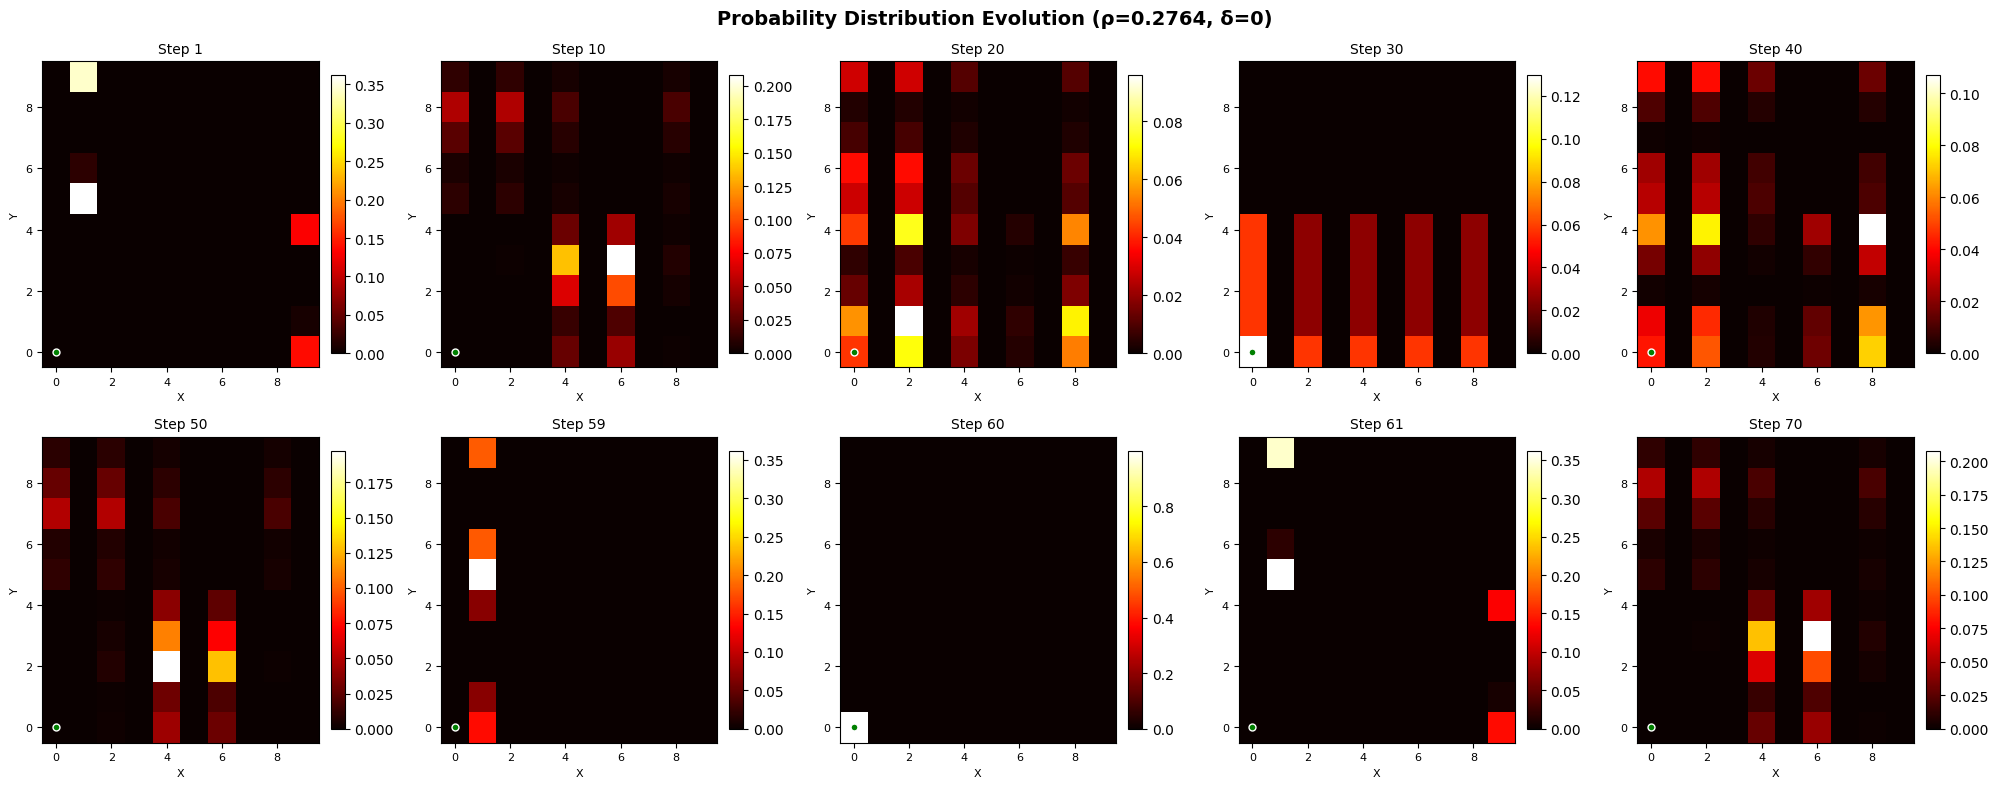
\includegraphics[width=\textwidth]{../fig-10x10-probability.png}
  \caption{Position probability distribution at ten snapshots between
           step~1 and step~70, for the same parameters as
           Fig.~\ref{fig:10x10-fidelity}. The walker starts localised at
           the origin, spreads outward over the first thirty steps, and
           refocuses to the origin at $N = 60$. The distribution at
           step~60 matches the initial condition; the distributions at
           intermediate steps do not.}
  \label{fig:10x10-probability}
\end{figure*}
